\documentclass[a4paper,oneside]{memoir}
\usepackage[english]{babel}
\usepackage[T1]{fontenc}
\usepackage[utf8]{inputenc}
\usepackage{wallpaper}
\usepackage{palatino}
\usepackage{listings}
\usepackage{hyperref}
\usepackage{float}
\usepackage{subcaption}
\usepackage{bm}
\usepackage{amsmath}
\hypersetup{
    colorlinks=true,
    linkcolor=blue,
    filecolor=magenta,      
    urlcolor=cyan,
}


\counterwithout{section}{chapter}
\counterwithout{figure}{chapter}
% Setup captions
%\captionstyle[\centering]{\centering}
%\changecaptionwidth
%\captionwidth{0.8\linewidth}

% Protect against widows and orphans
%\clubpenalty=10000
%\widowpenalty=10000

%\linespread{1.2}

%\raggedbottom

%\chapterstyle{ger}

%\maxsecnumdepth{subsection}

\lstset{language=C,
                basicstyle=\ttfamily,
                keywordstyle=\color{blue}\ttfamily,
                stringstyle=\color{red}\ttfamily,
                commentstyle=\color{green}\ttfamily,
                morecomment=[l][\color{magenta}]{\#}
}

\lstset{language=python,
                commentstyle=\color{red}\ttfamily,
}

%%  Setup fancy style quotation
%%  ==================================================================
%\usepackage{tikz}
%\usepackage{framed}

%\newcommand*\quotefont{\fontfamily{fxl}} % selects Libertine for quote font

% Make commands for the quotes
%\newcommand*{\openquote}{\tikz[remember picture,overlay,xshift=-15pt,yshift=-10pt]
%     \node (OQ) {\quotefont\fontsize{60}{60}\selectfont``};\kern0pt}
%\newcommand*{\closequote}{\tikz[remember picture,overlay,xshift=15pt,yshift=5pt]
%     \node (CQ) {\quotefont\fontsize{60}{60}\selectfont''};}

% select a colour for the shading
%\definecolor{shadecolor}{rgb}{1,1,1}

% wrap everything in its own environment
%\newenvironment{shadequote}% 
%{\begin{snugshade}\begin{quote}\openquote}
%{\hfill\closequote\end{quote}\end{snugshade}}

%%  Begin document
%%  ==================================================================
\begin{document}

%%  Begin title page
%%  ==================================================================
    \thispagestyle{empty}
    \ULCornerWallPaper{1}{ku-coverpage/diku-en.pdf}
    \ULCornerWallPaper{1}{ku-coverpage/diku-en.pdf}
    \begin{adjustwidth}{-3cm}{-1.5cm}
    \vspace*{-1cm}
    \textbf{\Huge Project outside course scope} \\
    \vspace*{2.5cm} \\
    \textbf{\Huge Accelerating Ocean Modelling} \\
    \vspace*{.1cm} \\
    {\huge Adressing performance bottlenecks of the ocean modelling framework Veros} \\
    \begin{tabbing}
    % adjust the hspace below for the longest author name
    Till Grenzdörffer \hspace{1cm} \= \texttt{vmt184@alumni.ku.dk} \\
    \\[12cm]
    \textbf{\Large Supervisor} \\
    Cosmin Eugen Oancea \> \texttt{cosmin.oancea@di.ku.dk} \\
    \end{tabbing}
    \end{adjustwidth}
    \newpage
    \ClearWallPaper



%%  ==================================================================
%%  End title page
\section{Introduction}
Currently many scientists are using purely sequential software for ocean modelling, leading to long simulation times and inefficient use of modern hardware. 
The aim of this project is to tackle this problem by introducing and optimizing highly parallel code that uses the potential of modern GPUs to accelerate the modelling process.

The ocean modelling framework this project is based on is Veros \cite{veros}. It is written in Python and uses Jax \cite{jax2018github} to parallelize large parts of the computations.
However, there is reason to believe that the parallel code generated by Jax (specifically on GPUs) is not optimal and warrants the implementation of specific bottlenecks in a language like CUDA, possibly generated by Futhark \cite{futhark}.

In this project I investigated two algorithms and one longer routine based on the Jax implementations from the Veros frameworks in order to find a performant solution.
Another contribution of this project is the integration of the resulting CUDA implementations into the Jax framework through XLA custom calls. This allows an easy use of the parallel code through a python interface.

In the first part I discuss different algorithms for solving tridiagonal systems, how they can be parallelized and how the choice of algorithm depends on the problem at hand. Afterwards I investigate the turbulent kinetic energy routine from the Veros framework for bottlenecks. The most important part of this routine is the Superbee scheme, on which I show the concept of \emph{overlapping tiles} for stencil computations.
The last part of this report focuses on the integration of CUDA code into Jax through XLA calls and shows how the different components interact with each other.


IN the end blah blah Jax vs CUda speed


\section{Tridiagonal Solver}
In this project I first investigated the implementation of a tridiagonal solver that is used throughout Veros. 
A tridiagonal system of size $n$ is shown in fig.~\ref{eq:tridiag}, where $\bm{a}$, $\bm{b}$ and $\bm{c}$ are vectors of size $n$ and $a_0 = c_n = 0$ 

The diagonals $\bm{a}$, $\bm{b}$ and $\bm{c}$, as well as $\bm{d}$ are given and the task of the solver is to find $\bm{x}$.

\begin{equation} \label{eq:tridiag}
    \begin{bmatrix}
        b_1 & c_1 & 0  & 0 & 0 & 0 & 0 & 0 \\
        a_2 & b_2 & c_2 & 0 & 0 & 0 & 0 & 0\\
        0   & a_3 & b_3 & c_3 & 0 & 0 & 0 & 0\\
        0   &  0  & a_4 & b_4 & c_4 & 0 & 0 & 0\\
        0   &  0  &  0  & a_5 & b_3 & \dots & 0  & 0\\
        0   &  0  &  0  &  0  & \dots & \dots &  \dots & 0 \\
        0   &  0  &  0  &  0  &  0  & \dots & \dots & c_{n-1}\\
        0   &  0  &  0  &  0  &  0  &  0  & a_n & b_n \\
    \end{bmatrix}
    \begin{bmatrix}
        x_1 \\
        x_2 \\
        x_3   \\
        x_4   \\
        \dots   \\
        \dots   \\
        \dots   \\
        x_n   \\
    \end{bmatrix}
     = 
     \begin{bmatrix}
        d_1 \\
        d_2 \\
        d_3   \\
        d_4   \\
        \dots   \\
        \dots   \\
        \dots   \\
        d_n   \\
    \end{bmatrix}
\end{equation}


The requirement for the solver in Veros is that it solves many (ca. 50000) tridiagonal systems of comparably small size (ca. 100) as fast as possible.

I considered two algorithms for solving tridiagonal systems for this task and experimented with different performance optimizations for both.

\subsection{Thomas Algorithm}
One simple algorithm for solving a tridiagonal system is the Thomas Algorithm.
Pythonlike pseudocode for it is shown in eq.~\ref{fig:thomas}, where a, b, c, d and x refer to the respective vectors shown in eq.\ref{eq:tridiag}.
We can see that in the both for-loops there are true RAW-dependencies across iterations, which means that the algorithm itself is not trivially parallelizable.
However, in our case we want to solve many small tridiagonal systems, so we can parallelize over the different systems and leave the Thomas Algorithm in its sequential form.
As long as we have enough systems to fully utilize the GPU it is running on, this implementation seems like a good approach.

\begin{figure}[hbtp]
    \caption{Thomas algorithm in pythonlike pseudocode}
    \label{fig:thomas}
    \begin{lstlisting}[language=python,frame=single]
for i in range(1, n):
    w = a[i] / b[i - 1]
    b[i] += -w * c[i - 1]
    d[i] += -w * d[i - 1]

x[-1] = d[-1] / b[-1]

for i in range(n - 2, -1, -1):
    x[i] = (d[i] - c[i] * out[i + 1]) / b[i]
    \end{lstlisting}
\end{figure}


\subsection{Thomas Algorithm - Coalesced}
\label{sec:thomas_coal}
In the trivial algorithm, successive iterations of the recurrent loop access neighboring data in memory.
Since we assign one tridiagonal system to each thread, neighboring threads access data with the stride of the size of the tridiagonal system. This means that the accesses are uncoalesced and we can improve the performance significantly by changing the underlying data layout. 
In this case the change is trivial - we just need to transpose the input matrix, which can be done efficiently using shared-memory tiling and tranpose the result back afterwards. 

Of course this is only beneficial if the time saved in the main kernel is larger due to coalesced access than the time spent tranposing the inputs and results.

\subsection{Thomas Algorithm - Loop unrolling}
Since in our use case the size of the tridiagonal systems is relatively small, it might make sense to unroll the recurrent loops. However, this is only possible if we know the size of the systems at compile time, or compile the CUDA kernel at runtime (for example using CuPy \cite{cupylearningsys2017}). 
However, I expect the benefit of this to be too small to warrant the significant overhead of JIT compilation.

\subsection{Flat version}
The flat version of the tridiagonal solver is based on the observation, 
that all recurrences in the Thomas algorithm can be replaced with a scan with an appropriate operator. 
For example, after inlining the computation of w and replacing the +=, we get the following line: 
\begin{verbatim}
    b[i] = b[i] - a[i] * c[i - 1] / b[i - 1] 
\end{verbatim}
As explained in \cite{andreetta2016finpar} in more detail, this statement matches the pattern $b_i = a_i + c_i / b_{i-1}$, which can be replaced with a scan that uses 2x2 matrix multiplication as its operator.
Similarly, the other recurrences can be replaced by a scan with linear function composition.
Fig.~\ref{fig:thomas_flat} shows the flattened futhark code for the first recurrence.
The other two recurrences are also composed of two map and one scan operation each, though with 2-tuples instead of 4-tuples and a different operator for the scan. Thus for the full algorithm 6 map and 3 scan operations are needed.

\begin{figure}[hbtp]
    \caption{First recurrence of the flattened tridiagonal solver in Futhark, taken from \cite{andreetta2016finpar}}
    \label{fig:thomas_flat}
    \begin{lstlisting}[language=haskell,frame=single]
let b0 = b[0]
let mats = map (\i: ->
                if 0 < i
                then (b[i], 0.0-a[i]*c[i-1], 1.0, 0.0)
                else (1.0,  0.0,             0.0, 1.0))
                (iota n)

let scmt = scan (\(a0,a1,a2,a3) (b0,b1,b2,b3) ->
                    let value = 1.0/(a0*b0)
                    in ( (b0*a0 + b1*a2)*value,
                        (b0*a1 + b1*a3)*value,
                        (b2*a0 + b3*a2)*value,
                        (b2*a1 + b3*a3)*value))
                (1.0,  0.0, 0.0, 1.0) mats

let b = map (\(t0,t1,t2,t3) ->
                    (t0*b0 + t1) / (t2*b0 + t3))
                scmt
    \end{lstlisting}
\end{figure}


I implemented this flat algorithm in CUDA using the thrust library, which provides a scan implementation with custom operators on the GPU.
For comparison, I also included the Futhark implementation of the authors of \cite{andreetta2016finpar} from the 
\href{https://github.com/diku-dk/futhark-benchmarks/blob/bf5112d0841866dc7370586f2e2a7b48467d2d97/finpar/LocVolCalib.fut}{futhark benchmarks}
repository.

Compared to the Thomas algorithm, this algorithm is more computationally expensive, however if the size of the tridiagonal systems is large enough or we have sufficiently parallel hardware, the benefits of parallelization should outweigh the additional computational load.

\subsection{Flat version - shared memory}
Since my initial implementation of the flat algorithm used thrust scans, the computation involved the launch of 6 kernels in total. This means that there are a lot of redundant accesses to global memory. 

In order to evaluate the effect of this, I also implemented a version of the flat algorithm that is computed completely within shared memory.

Here a block is assigned to each tridiagonal system (given that the system is not too large to fit shared memory), and the flat algorithm is computed using intra block scans. For this I used parts of the code handouts from the PMPH course.


\subsection{Precision}
In order to be useful, all of the implementations of course need to produce results that match a reference implementation. However, due to the nature of floating point computation, this will almost never be exact.

Interestingly, the error margin varied a lot between the algorithms. The flat implementations suffered far greater imprecision, probably at least partly due to the increased parallelism and thereby more indeterminstic order of execution, but also just due to the higher number of floating point calculations.

However, in Veros the tridiagonal systems this solver is supposed to work on are guaranteed to be diagonally dominant. Testing the algorithms on systems with this property showed that all algorithms produce meaningful results.
\subsection{Futhark}
In addition to the CUDA implementations, I also included a sequential and a flat implementation (from \href{https://github.com/diku-dk/futhark-benchmarks/blob/bf5112d0841866dc7370586f2e2a7b48467d2d97/finpar/LocVolCalib.fut}{futhark benchmarks}) in the benchmarks in order to see how close the high level description of the algorithms compiled by the futhark compiler will come to CUDA implementations that were optimized by hand.

\subsection{Benchmarks}

\vspace*{\fill}

\begin{figure}[H]
    \begin{subfigure}[b]{0.6\textwidth}
        \centering
        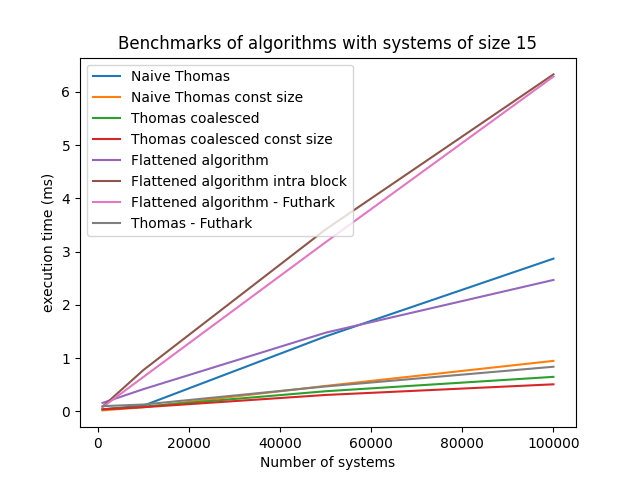
\includegraphics[width=\textwidth]{timings_15.png}
        \caption{Tridiagonal systems of size 15}
        \label{fig:bench15}
    \end{subfigure}
    % \hfill
    \begin{subfigure}[b]{0.6\textwidth}
        \centering
    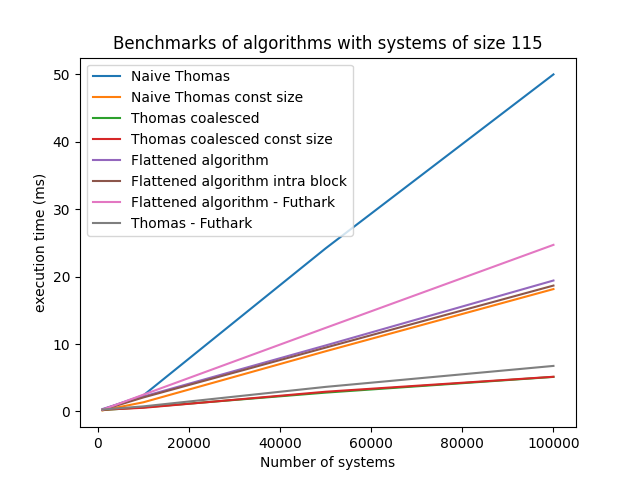
\includegraphics[width=\textwidth]{timings_115.png}
    \caption{Tridiagonal systems of size 115}
    \label{fig:bench115}
        \end{subfigure}
    % \vskip\baselineskip
    \begin{subfigure}[b]{0.6\textwidth}
        \centering
    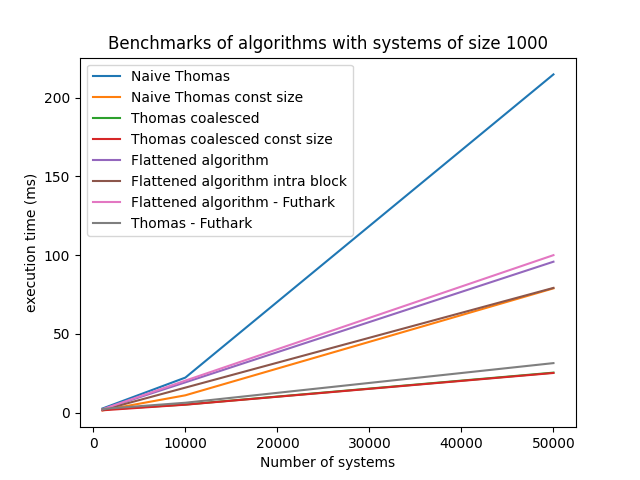
\includegraphics[width=\textwidth]{timings_1000.png}
    \caption{Tridiagonal systems of size 1000}
    \label{fig:bench1000}
    \end{subfigure}
    % \hfill
    \begin{subfigure}[b]{0.6\textwidth}
        \centering
    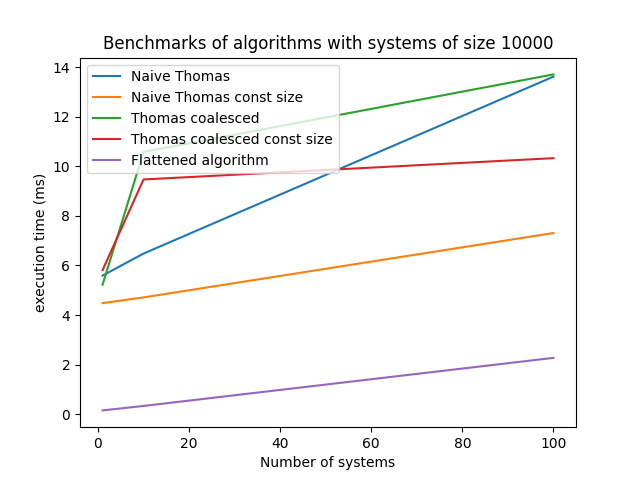
\includegraphics[width=\textwidth]{timings_10000.png}
    \caption{Tridiagonal systems of size 10000}
    \label{fig:bench10000}
    \end{subfigure}
    
 \end{figure}

The performance of the different algorithms are shown in figs.~\ref{fig:bench15}-\ref{fig:bench10000}. All benchmarks were executed on a RTX 2070 Super GPU. 
The algorithms were tested on a different number of systems, and on systems of sizes 15, 115, 1000 and 10000. In our target application the size 115 is the most relevant and the algorithms should perform well on ca. 50000 systems.

In fig.~\ref{fig:bench15} we can see that for small systems the flat algorithms are not performing very well. Because of the small size of the systems, the overhead for parallelizing the recurrences outweighs the benefits of the parallelization.

The sequential algorithms perform similarly well, though it is noteworthy that the performance of the uncoalesced Thomas algorithm with compile-time known size of the systems performs almost on par with the coalesced versions. The small stride of 15 still leads to decent locality of reference and the transpositions needed for the coalesced versions could make up the rest of the difference.

For our target system size of 115 we can see that the naive Thomas implementation performs by far the worst. The flattened versions now achieve a similar performance as the trivial Thomas algorithm with compile-time know size.
The best performance is shown by the coalesced versions, independant of whether the size of the systems is known at compile time. However, the futhark implementation follows right behind. It is important to mention here that the futhark implementation does not contain any special instructions that would result in coalesced access. The futhark compiler deduced the need of transpositions itself and came up with a solution that almost matches hand-optimized CUDA code.

With systems of size 1000 we see the same pattern as for size 115. Apparanetly the systems are still not large enough to reap the benefits of the increased parallelism (at least on the machine used). However, we can see a noticable improvement in performance by the intra block flat version as compared to the implementation that uses thrust. The use of shared memory to avoid global memory accesses starts to pay off.

Lastly, I tested the algorithms on smaller batches of large systems of size 10000. Here the best implementation is indeed the flat version. The sequential version are all similarly slow. The sharp bend in the performance of the coalesced versions is due to the transposition being a no-op for a single system.
The futhark and intra block implementations are not included here, since the systems were too large to fit into shared memory. 

\subsection{Conclusion}
For this particular application (and the hardware I tested the algorithms on) we can see that due to the small size of the tridiagonal systems it makes most sense to have an algorithm that works sequentially on each of the systems and optimizes the memory layout such that this algorithm can be executed on many systems in parallel. 

The flattened algorithm make sense in other cases though. If there are few or even only a single large tridiagonal system to solve, they outperform the sequential approach. If the system is small enough to fit into shared memory we can compute the solution within a single kernel call. 

We can see that there are lots of parameters that influence which solution is the most optimal. Thus we can use apply incremental flattening \cite{incremental} here to compile different versions of the algorithm and choose dynamically, which version is going to be executed, depending on system capabilities and the size of the problem.



\section{Turbulent kinetic energy}
After integrating the tridiagonal solver into Jax (see section~\ref{sec:integrate}), I decided to look at one example context in which the solver would be used.

The turbulent kinetic energy benchmark is a larger routine that uses different components like the tridiagonal solver. It acts on a three dimensional grid and contains a lot of stencil computations.

This routine is responsible for qunatifying the effect of small-scale water turbulence on the overall state of the simulation. Since we work on a discrete grid with a fixed resolution, effects that occur within one grid cell will not be taken into account. Thus it is important to use the quantifcation of this effect, offered by the turbulent kinetic energy routine, such that these turbulence do not need to be calculated in detail.

\subsection{Components}
The turbulent kinetic energy routine mainly consists of the following parts:
\begin{enumerate}
    \item Initializing a lot of tridiagonal systems
    \item Solving these systems 
    \item Multiple 2D stencil operations
    \item The Superbee scheme
\end{enumerate}
After integrating my tridiagonal solver and profiling the benchmark using tensorboard, which is well supported by Jax, I found that the Superbee scheme was the largest bottleneck.  




\subsection{Superbee scheme}
The superbee scheme is part of a stencil calculation that also works on a 3D grid.
Its purpose is to calculate the influence of advection of tracers within the water and will result in three values for each of the grid cell. One value corresponding to flux along the first dimension of the grid (named flux\_east), one along the second dimension (named flux\_north) and one along the third dimension (named flux\_top).

Since I do not have sufficient knowledge of the physics and mathematics behind this operation, I looked at this problem purely from a coding perspective. More specificly I tried to understand the pattern of memory accesses and tried to map the computation efficiently to CUDA code.

The indexing pattern of the stencil is shown in fig.~\ref{fig:stencil_code} and a 2D projection of it is visualized in fig.~\ref{fig:stencil_shape}. 

\begin{figure}[hbtp]
    \caption{Superbee stencil access pattern}
    \label{fig:stencil_code}
    \begin{lstlisting}[language=python,frame=single]
for x in range(width):
    for y in range(height):
        for z in range(depth):
            flux_east[x,y,z] =  f(grid[x-2,y,z], 
                                  grid[x-1,y,z],
                                  grid[x,  y,z],
                                  grid[x+1,y,z])

            flux_north[x,y,z] = f(grid[x,y-2,z], 
                                  grid[x,y-1,z],
                                  grid[x,y,  z],
                                  grid[x,y+1,z])

            flux_top[x,y,z] =   f(grid[x,y,z-2], 
                                  grid[x,y,z-1],
                                  grid[x,y,z  ],
                                  grid[x,y,z+1])
    \end{lstlisting}
\end{figure}
\begin{figure}[h]
    \centering
    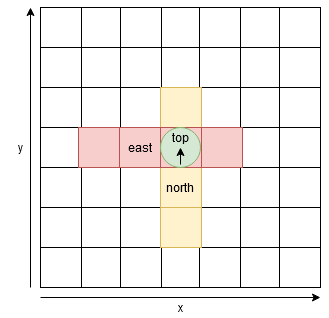
\includegraphics[width=0.5\textwidth]{stencil.png}
    \caption{2D projection of the stencil shape. The green dot symbolizes the flux in "top" direction, going along the z axis.}
    \label{fig:stencil_shape}
\end{figure}

A very straightforward observation about this pattern is, that there is an overlap of the three computations. This means that when implementing this scheme in CUDA it makes sense to fuse the computations together, such that the value $grid\left[x,y,z\right]$ only has to be read once from global memory and can be stored in registers.

\subsubsection{Tiled stencil computation}
In order to save more accesses to global memory, we can observe that successive iterations of this stencil computation will also read almost the same data.
For example, in the iteration $x = 0 ; y = 0 ; z = 2$ we read $grid[0,0,0]$, $grid[0,0,1]$,$grid[0,0,2]$ and $grid[0,0,3]$ and in iteration $x = 0 ; y = 0 ; z = 3$
we read $grid[0,0,1]$, $grid[0,0,2]$,$grid[0,0,3]$ and $grid[0,0,4]$. We can see that 75\% of the memory locations are shared between the iterations.

In order to use this to our advantage, we need to make use of shared memory.
By tiling the loops and loading 3D blocks of the data into shared memory, we can avoid a lot of global memory accesses. This \emph{overlapped tiling} approach is described in \cite{stencil_lift}.
Pseudocode for the tiled approach is shown in fig.~\ref{fig:stencil_tiled}.

\begin{figure}[hbtp]
    \caption{Tiled Superbee stencil}
    \label{fig:stencil_tiled}
    \begin{lstlisting}[language=python,frame=single]
for xx in range(0, width, TILE_SIZE):
    for yy in range(0, height, TILE_SIZE):
        for zz in range(0, depth, TILE_SIZE):
            # load block grid[xx-2:xx+TILE_SIZE+1, 
            #                 yy-2:yy+TILE_SIZE+1,
            #                 zz-2:zz+TILE_SIZE+1]
            # to shared memory in coalesced fashion
            shared_memory[...] = grid[...]
            for x in range(TILE_SIZE):
                for y in range(TILE_SIZE):
                    for z in range(TILE_SIZE):
    # wrong indentation so code fits the page
    # all below this is inside all loops     
                flux_east[x,y,z] =  f(grid[x-2,y,z], 
                                      grid[x-1,y,z],
                                      grid[x,  y,z],
                                      grid[x+1,y,z])

                flux_north[x,y,z] = f(grid[x,y-2,z], 
                                      grid[x,y-1,z],
                                      grid[x,y,  z],
                                      grid[x,y+1,z])

                flux_top[x,y,z] =   f(grid[x,y,z-2], 
                                      grid[x,y,z-1],
                                      grid[x,y,z  ],
                                      grid[x,y,z+1])
    \end{lstlisting}
\end{figure}

We can see that there are still some redundant loads on the border of the tiles, however if the tile is large enough these are negligible. 

Loading the grid data to shared memory in coalesced fashion is not exactly trivial, since there is a mismatch between the number of threads that are loading the data ($TILE\_SIZE^3$) and the number of entries to be loaded from global memory: $(TILE\_SIZE+3)^3$.

\subsection{Turbulent Kinetic Energy in Futhark}
After further profiling of the turbulent kinetic energy Jax implementation with custom operations for the tridiagonal solver and the superbee scheme, it became apparent that most of time is not spent on computation. A lot of gather operations were performed, each in a seperate kernel, which led to the assumption that a lot of arrays are created for intermediate results. Most of these operations seemed to correspond to array slicing which was used extensively in the Jax code. 

To check this hypothesis I implemented the full routine in Futhark. 
Interestingly, the futhark code (compiled to opencl) ran slightly slower than the Jax code with GPU backend. However, after using Futhark's autotune feature the program sped up by a factor of 4, outperforming Jax by a huge margin. This again shows the importance of the use of incremental flattening to match the problem proportions and the available hardware resources.


\subsection{Benchmarks}
\section{Interfacing with Jax}
\label{sec:integrate}
In order to use the optimized CUDA code within the Veros framework, I decided to use the wrappers around Tensorflow's \cite{tensorflow} XLA Custom Calls that are provided by the Jax library. The custom calls are used to encapsulate native code and directly pass pointers to device memory, which can then be read and written by the CUDA kernels. The whole pipeline is shown in fig.~\ref{fig:integration}.

An interesting feature of the XLA custom call API is the option to define a memory layout for the data passed to the native code. We can use this for the implementation of the tridiagonal solver. In the python routines that use the tridiagonal solver the systems are stored in such a way that consecutive elements of one diagonal are stored consecutively in memory and all $n$ systems are stored one after the other. However with the custom calls we can decide to store consecutive elements with a stride of $n$, effectively transposing the input and allowing for coalesced access with the implementation of the Thomas algorithm shown in section \ref{sec:thomas_coal}.

\begin{figure}[h]
    \centering
    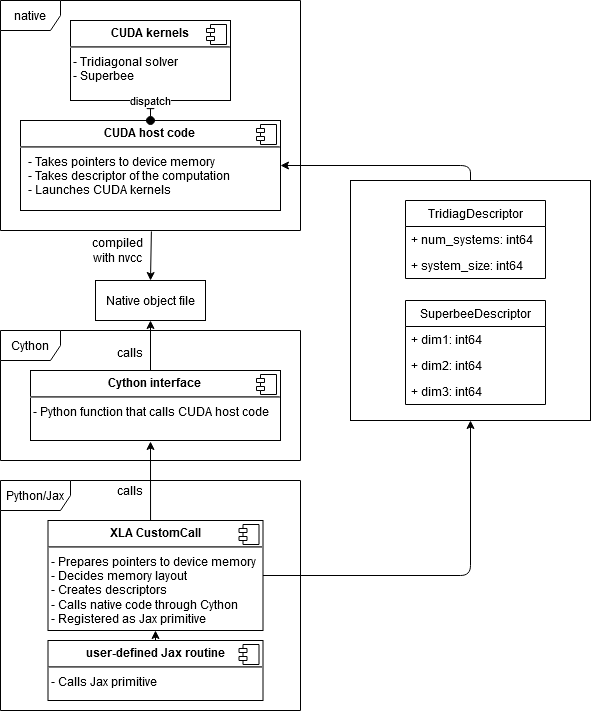
\includegraphics[width=\textwidth]{integration.png}
    \caption{Interaction between Jax, Cython and CUDA.}
    \label{fig:integration}
\end{figure}

% Uses XLA
% Integrating CUDA code with Cython
% Needs modified compiler... blah



\bibliographystyle{ieeetr}
\bibliography{main}
\end{document}
%%  ==================================================================
%%  End document
\iffalse %project description

Currently, many scientists use purely sequential software for ocean modelling, leading to long simulation times andinefficient use of modern hardware.The aim of this project is to tackle this problem by introducing highly parallel code that uses the potential of modern GPUsto accelerate the modelling process.Specifically the student will try to enhance the performance of the library Veros using massively GPUs.In this library there exist a few specific bottlenecks that significantly slow down the modelling process. For example,since the modelling process uses a grid-like structure, there is the need to quantify the effect of water turbulence thatis a lot smaller than one grid cell on the large-scale flow of the ocean.This problem and another two of the most important bottlenecks are already implemented using different performance-focused frameworks like JAX, Numba, CuPy, etc. with the aim of finding a suitably performant solution. However, thereis hope that these implementations can be improved further or that other languages like CUDA and Futhark can yieldhigher performance gains.Within the project, the student implements these bottlenecks in the GPU-accelerated languages CUDA and Futhark,aiming to achieve a solution that performs better than the existing implementations. This can potentially save a lot of timefor the scientists running the experiments and possibly also reduce the energy consumption required for the modellingprocess by using the hardware more efficiently.This involves interfacing the new implementations with the existing codebase, more specifically with the frameworkJAX, through either passing pointers to the GPU memory between the libraries or registering XLA “custom calls” withJAX. These XLA “custom calls” would allow the direct use of C++ or CUDA code (possibly generated by Futhark) withinJAX.Additionally this project requires the use of profiling tools for evaluating the performance of the implementations as wellas potentially identifying further bottlenecks in the framework.Learning Goals:• Understanding the basic structure of the ocean modelling library Veros• Efficient algorithm design in different parallel languages (CUDA/Futhark)• Identification of performance bottlenecks in parallel programs• Interfacing Futhark and CUDA implementation with existing python codebases• Using XLA custom calls to use C++/CUDA code within JAX*29/01/2021WrittenAccelerating Ocean Modelling
\fi